\documentclass[a4paper, 14pt]{extarticle}
\usepackage[russian]{babel}
\usepackage[T1]{fontenc}
\usepackage{fontspec}
\usepackage{indentfirst}
\usepackage{enumitem}
\usepackage{graphicx}
\usepackage[
  left=20mm,
  right=10mm,
  top=20mm,
  bottom=20mm
]{geometry}
\usepackage{parskip}
\usepackage{titlesec}
\usepackage{xurl}
\usepackage{hyperref}
\usepackage{float}
\usepackage[
  figurename=Рисунок,
  labelsep=endash,
]{caption}
\usepackage[outputdir=build, newfloat]{minted}

\hypersetup{
  colorlinks=true,
  linkcolor=black,
  filecolor=blue,
  urlcolor=blue,
}

\renewcommand*{\labelitemi}{---}
\setmainfont{Times New Roman}
\setmonofont{JetBrains Mono}[
  SizeFeatures={Size=11},
]

\newenvironment{code}{\captionsetup{type=listing}}{}
\SetupFloatingEnvironment{listing}{name=Листинг}

\setminted{
  fontsize=\footnotesize,
}

\setlength{\parskip}{6pt}

\setlength{\parindent}{1cm}
\setlist[itemize]{itemsep=0em,topsep=0em,parsep=0em,partopsep=0em,leftmargin=2.0cm,wide}
\setlist[enumerate]{itemsep=0em,topsep=0em,parsep=0em,partopsep=0em,leftmargin=2.0cm,wide}

\renewcommand{\thesection}{\arabic{section}.}
\renewcommand{\thesubsection}{\thesection\arabic{subsection}.}
\renewcommand{\thesubsubsection}{\thesubsection\arabic{subsubsection}.}

\titleformat{\section}{\normalfont\bfseries}{\thesection}{0.5em}{}
\titleformat{\subsection}{\normalfont\bfseries}{\thesubsection}{0.5em}{}

\titleformat*{\section}{\normalfont\bfseries}
\titleformat*{\subsection}{\normalfont\bfseries}

\linespread{1.5}
\renewcommand{\baselinestretch}{1.5}

\begin{document}

\begin{titlepage}
  \vspace{0pt plus2fill}
  \noindent

  \vspace{0pt plus6fill}
  \begin{center}
    Санкт-Петербургский национальный исследовательский университет
    информационных технологий, механики и оптики

    \vspace{0pt plus3fill}

    Факультет инфокоммуникационных технологий

    Направление подготовки 11.03.02

    \vspace{0pt plus2fill}

    Лабораторная работа №3

    <<Создание XML документов>>

  \end{center}

  \vspace{0pt plus6fill}
  \begin{flushright}
    Выполнил: \\
    Швалов Даниил Андреевич

    Группа: К33211

    Проверила: \\
    Марченко Елена Вадимовна
  \end{flushright}

  \vspace{0pt plus5fill}
  \begin{center}
    Санкт-Петербург

    2024
  \end{center}
\end{titlepage}

\section{Введение}

\textbf{Цель работы}: создать XML-документы.

\section{Ход работы}

\subsection*{Упражнение №1. Создание простого XML-документа}

В данном упражнении необходимо создать XML-документ, описывающий данные
кандидатов на вакантную должность. При этом, документ должен содержать поля со
следующей информацией:
\begin{itemize}
  \item идентификатор кандидата;
  \item имя;
  \item фамилия;
  \item отчество;
  \item возраст;
  \item текущее место работы;
  \item занимаемая в данный момент должность;
  \item дата рождения;
  \item образование;
  \item адрес;
  \item телефон;
  \item семейное положение;
  \item желаемый оклад в рублях.
\end{itemize}

В качестве основы был взят документ, предоставленный вместе с описанием
лабораторной работы. Он был несколько изменен: в поле возраста для всех
кандидатов был установлен возраст на момент мая 2024 года. На рисунке
\ref{fig:task-1:1} представлен получившийся XML-документ.

\begin{figure}[H]
  \centering
  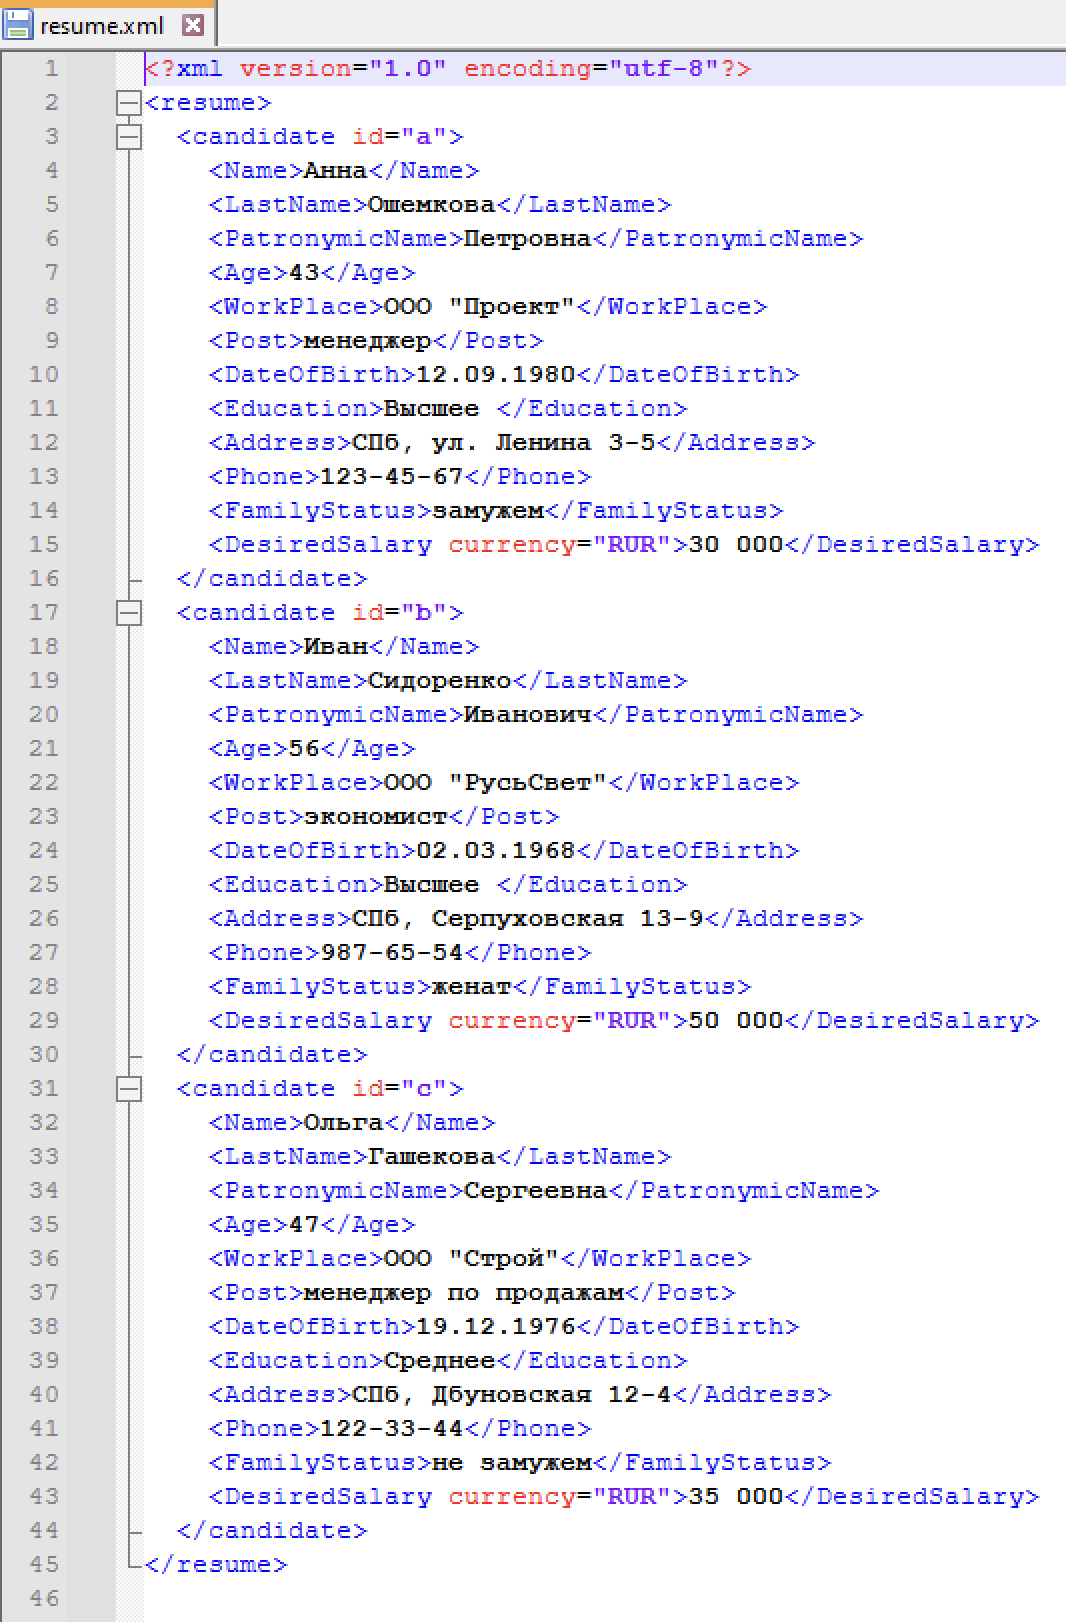
\includegraphics[width=0.7\textwidth]{images/task-1/1.png}
  \caption{XML-документ \textit{\foreignlanguage{english}{resume.xml}}}
  \label{fig:task-1:1}
\end{figure}

С помощью плагина XML Tools в Notepad++ получившийся XML-документ был
проверен на корректность (рисунок \ref{fig:task-1:2}). Как видно на рисунке
\ref{fig:task-1:3}, XML-документ является корректным.

\begin{figure}[H]
  \centering
  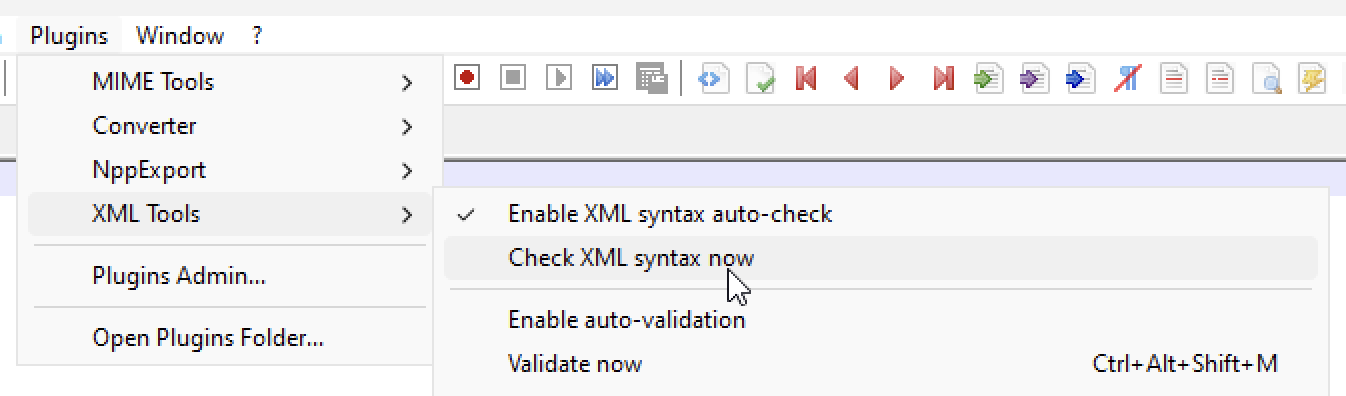
\includegraphics[width=0.8\textwidth]{images/task-1/2.png}
  \caption{Кнопка проверки XML-документа на корректность}
  \label{fig:task-1:2}
\end{figure}

\begin{figure}[H]
  \centering
  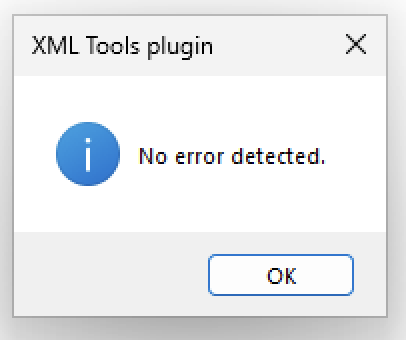
\includegraphics[width=0.3\textwidth]{images/task-1/3.png}
  \caption{Диалог, сообщающий об отсутствии ошибок}
  \label{fig:task-1:3}
\end{figure}

\subsection*{Упражнение №2. Создание XML-документа}

В данном упражнении необходимо создать XML-документ с описанием плана дисциплин.
В процессе анализа учебных дисциплин были выявлены следующие сущности:
\begin{itemize}
  \item \textbf{lessons}: сущность, представляющая список дисциплин.
  \item \textbf{lesson}: сущность, представляющая конкретную дисциплину.
  Содержит название дисциплины, фамилию преподавателя, номер семестра,
  количество академических часов, тип контроля и формат проведения. Также
  обладает уникальным идентификатором.
  \item \textbf{CourseName}: сущность, представляющая название дисциплины.
  \item \textbf{ProfessorSurname}: сущность, представляющая имя преподавателя,
  который проводит данную дисциплину.
  \item \textbf{Semester}: сущность, представляющая номер семестра, в котором
  проводится дисциплина.
  \item \textbf{AcademicHours}: сущность, представляющая количество
  академических часов данной дисциплины.
  \item \textbf{ControlType}: сущность, представляющая тип контроля (например,
  экзамен или зачёт).
  \item \textbf{Format}: сущность, представляющая формат проведения дисциплины
  (например, очный или дистанционный).
\end{itemize}

В итоге был составлен XML-документ, показанный на рисунке \ref{fig:task-2:1}.
Для примера были добавлены три дисциплины с различными значениями для таких
полей как формат проведения, тип контроля, количество академических часов и
номер семестра, в котором проводится дисциплина.

\begin{figure}[H]
  \centering
  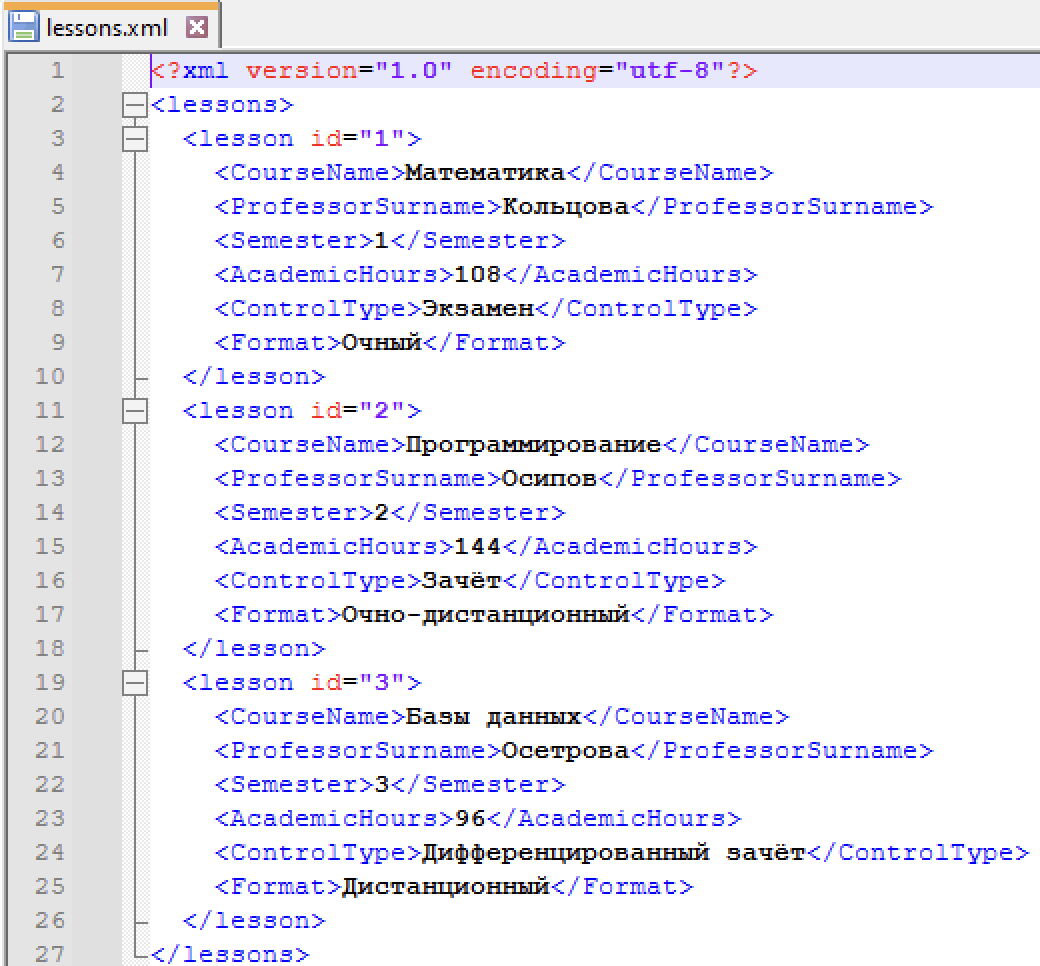
\includegraphics[width=0.7\textwidth]{images/task-2/1.png}
  \caption{XML-документ \textit{\foreignlanguage{english}{lessons.xml}}}
  \label{fig:task-2:1}
\end{figure}

\subsection*{Упражнение №3. Создание XML-документа}

В данном упражнении необходимо создать XML-документ на свободную тему. В данный
момент на дисциплине <<Разработка баз данных>> наша команда разрабатывает базу
данных на тему книг. Поэтому было принято решение создать XML-документ, хранящий
информацию о книгах.

В ходе анализа предметной области были выявлены следующие сущности:
\begin{itemize}
  \item \textbf{books}: сущность, представляющая список всех книг.
  \item \textbf{book}: сущность, представляющая конкретную книгу. Содержит
  заголовок, аннотацию, автора, жанр, количество страниц, язык издания,
  издательство, год издания, ISBN и возрастное ограничение. Также имеет
  уникальный идентификатор.
  \item \textbf{title}: сущность, представляющая заголовок книги.
  \item \textbf{summary}: сущность, представляющая аннотацию к книге.
  \item \textbf{authors}: сущность, представляющая авторов книги.
  \item \textbf{author}: сущность, представляющая конкретного автора книги.
  \item \textbf{genres}: сущность, представляющая жанры книги.
  \item \textbf{genre}: сущность, представляющая конкретный жанр книги.
  \item \textbf{pages}: сущность, представляющая количество страниц.
  \item \textbf{language}: сущность, представляющая язык, на котором издана
  книга.
  \item \textbf{publisher}: сущность, представляющая издательство.
  \item \textbf{publication\_year}: сущность, представляющая год издания книги.
  \item \textbf{isbn}: сущность, представляющая ISBN книги.
  \item \textbf{age\_limit}: сущность, представляющая возрастное ограничение
  книги.
\end{itemize}

Исходя из данных сущностей, был составлен XML-документ, представленный на
рисунке \ref{fig:task-3:1}.

\begin{figure}[H]
  \centering
  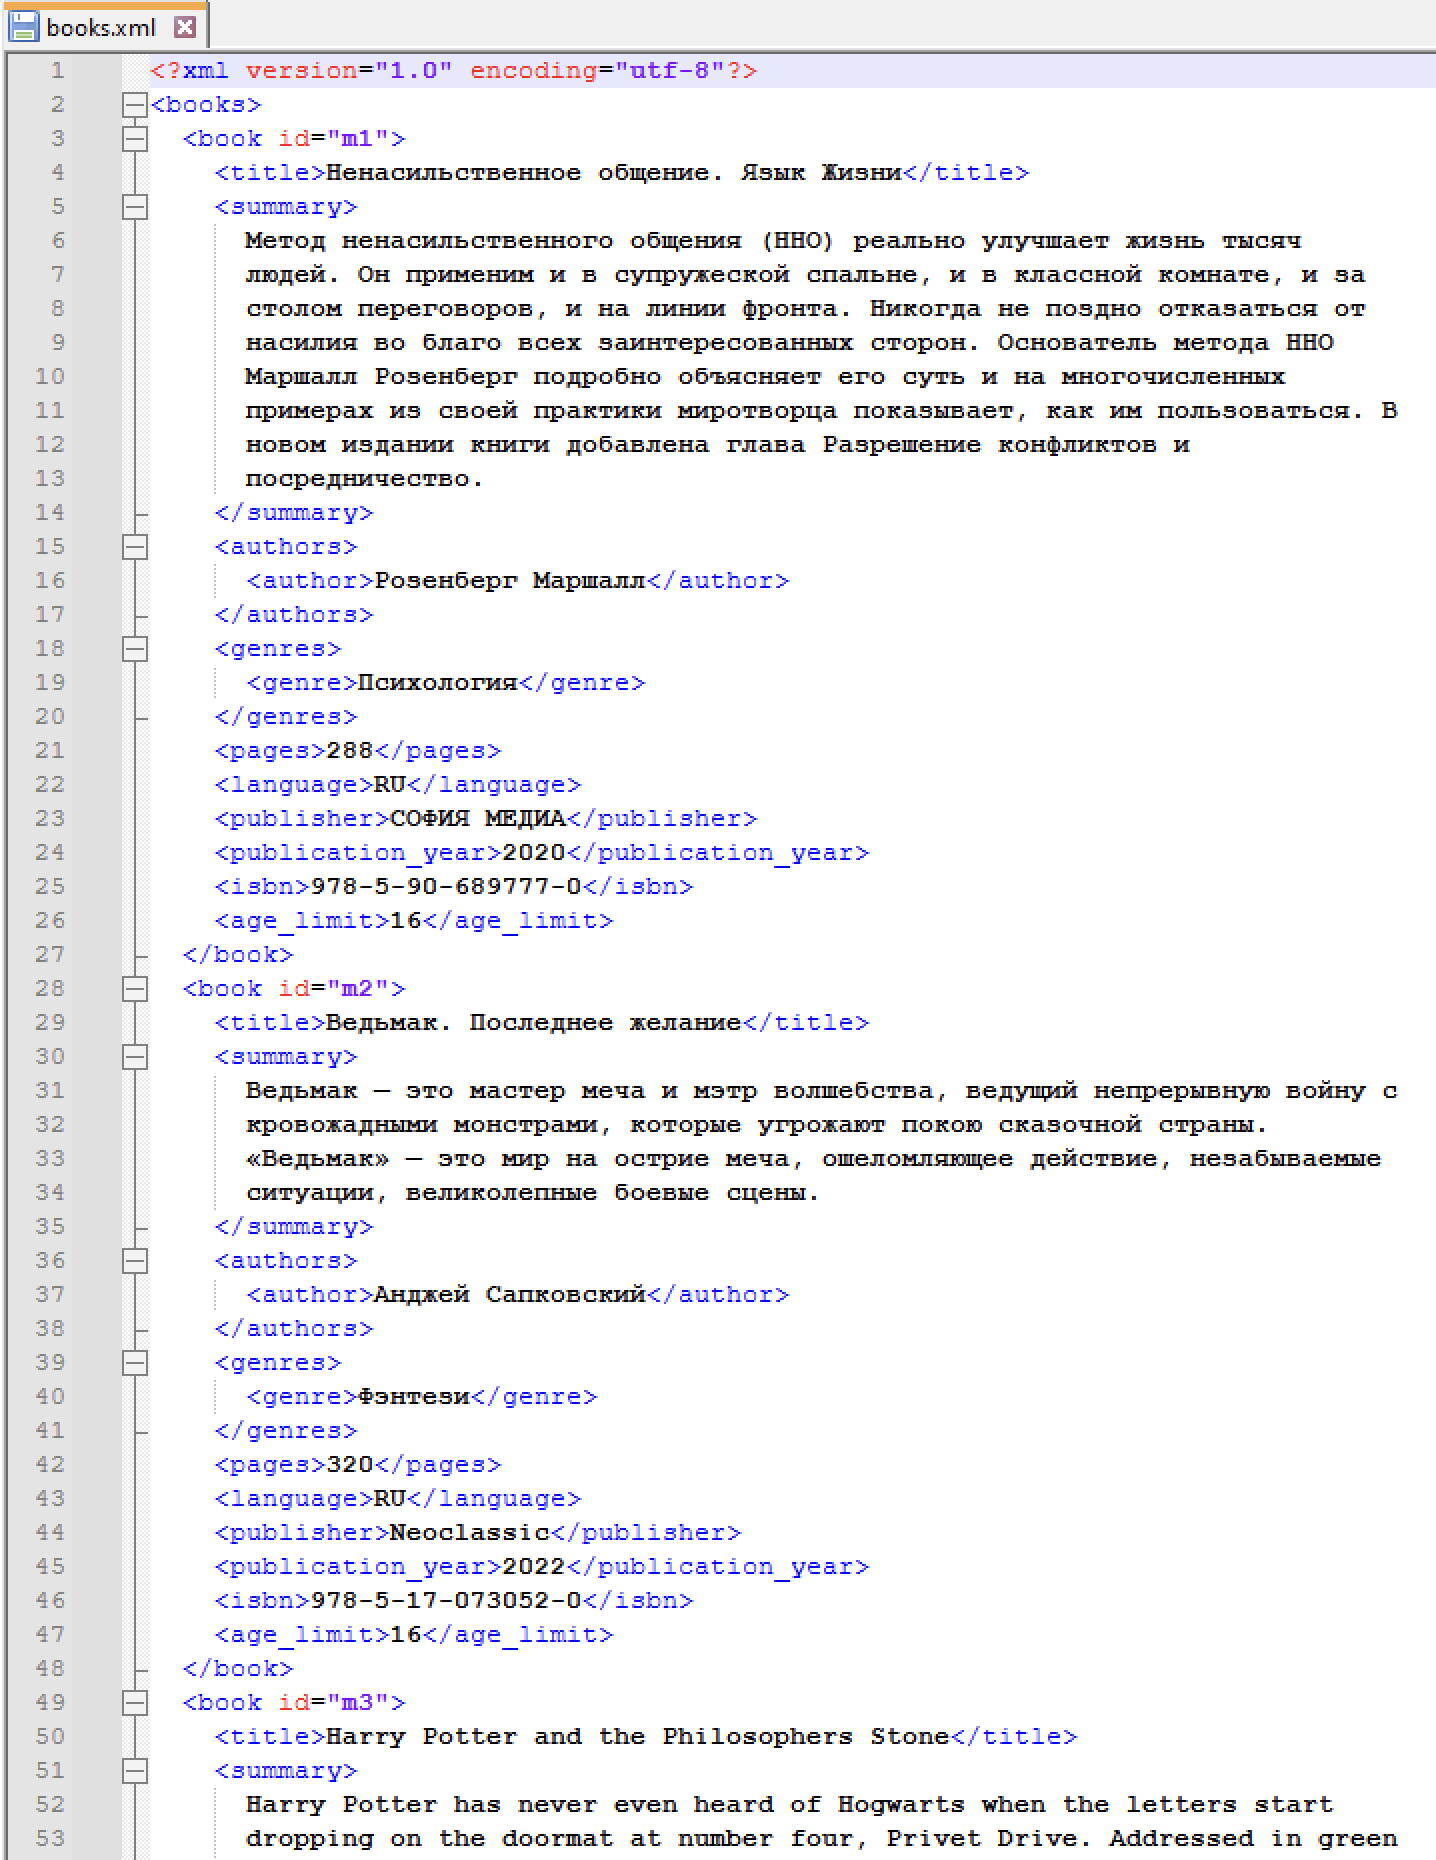
\includegraphics[width=0.7\textwidth]{images/task-3/1.png}
  \caption{XML-документ \textit{\foreignlanguage{english}{books.xml}}}
  \label{fig:task-3:1}
\end{figure}

\section{Вывод}

В ходе выполнения лабораторной работы были созданы XML-документы.

\end{document}
